
\providecommand{\myrootdir}{..}
\documentclass[\myrootdir/main.tex]{subfiles}

\begin{document}

\chapter{The Failing Build Logs Data Set}
\includegraphics[page=5, width=\textwidth, trim={0.5cm 0.5cm 0.5cm 0.5cm}, clip]{img/flow-of-research.pdf}

\label{sec:data-set}
\section{Motivation}
originally: log collection to get impression of build logs from various projects, what possibly extractable information they contain and how structured or unstructured they are.
Then labeling of one build log information, namely the reason the build failed, as well as keywords and structural category to use in our evaluation and support our impressions about suitability of the techniques with quantitative results

\section{Related Data Sets}
\todo{kind of related work for data set? the two mortiz sent, more?}

\section{Log Collector}
To collect a broad range of build logs we built the \texttt{Log Collector} using ruby.

\subsection{Sampling Repositories}
Our first task was to determine a set of repositories to query logs from.
Our \texttt{GHTorrentParser} can query the GHTorrent~\cite{gousios2013ghtorrent} data set for the most popular languages on github and the most popular repositories for a given language.
\emph{Popularity} in this case is defined as the number of watches.
Our \texttt{TravisRequester} can then check for a given repository whether it uses Travis CI.

\subsection{Sampling Builds}
The \texttt{LogCollector} uses the \texttt{TravisRequester}, our tool querying the Travis API~\cite{travisci2019apidoc}, to obtain the newest builds for a given repository.
As most builds on Travis CI are successful \mention{citation needed} we use a stratified sampling approach: \texttt{TravisRequester} saves the found builds in logs in buckets according to their state.
We encountered the following states during our data collection passes:
\begin{itemize}
	\item \todo{fill /5 mins/}
\end{itemize}
\texttt{TravisRequester} saves up to a configured number of builds per state and searches through a configured number of maximum checked builds.

\subsection{Sampling Logs}
For each build the \texttt{TravisRequester} then selects a log to download.
Logs in Travis CI are not directly attributed to \texttt{build}s, but to \texttt{job}s.
A single build can consist of multiple jobs, e.g.\ building and executing tests in various different testing environments.
\texttt{TravisRequester} therefore queries each build for a job, which has the same state.
A failed build can have successful job executions, as just one failed job leads to the whole build being marked as failed.
For the selected jobs, our tool then queries the Travis API V3 and obtains the respective build log.

\todo{image! like in travistorrent paper, /draft 10 mins/}

\section{Collection Process}
For our initial data collection to get an impression of build logs from various projects and languages we used the \texttt{LogCollector} to gather from the 30 most popular languages, up to 3 repositories using Travis CI each and 3 logs per state for each of those repositories.
For the \emph{Failing Build Log Data Set} we again collected from the same selection of repositories though saved only 10 logs of the state \emph{failed} for each repository.
our impression?
\todo{image!}


\section{Build Failure Reason}
\todo{WHY? one common information developers and researches might want to extract, intentionally not focus on one structurally clearly defined retrieval   cause that would be simple for PROSE retrieval -> better comparability}


\section{Data Model}
For our study, described in Chapter \ref{sec:study}, we want to investigate the retrieval capabilities of three techniques. Therefore, we need a data set of in/output examples for one \texttt{BuildLogInformation}. Furthermore, Keyword search is not configured by such in/output, but search keywords surrounding the desired output. Finally, this section describes our notion of structural categories, which we use to quantify our assumptions on the needed uniformness of in/output examples.

\subsection{Example Set}
Our data set is organized in example sets. One example set always contains build log in/output examples from the same software repository or project and for one specific build log information. They are all from one repository because we investigate information retrieval techniques which are always configured to the scope of one particular software repository or project.
Each example set has an identifying \emph{save name}, a \emph{build log information} that is desired to be extracted by this configuration, and a list of \emph{in / output examples}.

\subsection{In / Output Example}
In/output examples (I/O examples) are used to configure two of the information retrieval techniques we are evaluating for this thesis, PROSE regular expression program synthesis by example and text similarity.
In our data set they always consist of an \emph{input path}, linking to the build log file which is the input for this example.
The \emph{output} is a substring of that build log, the textual representation of the targeted build log information within the input build log.

\subsection{Keywords}
The keyword search is configured by a list of keywords which are searched in the document with plain text search.
In order to compare it to the two other techniques, each in/output example is associated with a list of 1 - 3 keywords that can be found close to the textual representation of the targeted build log information.

\paragraph{Description}
\todo{for simple keyword search - imitate what users would search for ad-hoc}

\todo{learning steps combining keywords -> similar to how devs would learn from reading those models}

\subsection{Categories}
Our intuition was that the ability of PROSE to be able to successfully learn a regex program depended on the structural uniformity of the provided in/output examples.
The regular expressions need a consistent pattern in the build log string at the borders or around the textual representation of a build log information to match on for the retrieval.
To be able to quantify this intuition in our evaluation we assigned \emph{structural categories} to each of the examples within an example set.
If two retrievals are at the same structural location with the build log, meaning they are surrounded by a similar markings, the fall into the same category.
For most cases, two build failure reason examples which fall into one category are outputted either within the same build step or by the same build step tool.

\section{Labeling}
\subsection{Output Examples: Build Failure Reason}
We labeled the first occuring substring describing the failure.
If there were multiple errors described we took the first continuous block of error description.

The labeler read or skimmed through build log and copy out the substring describing the reason the build failed.
Whitespace or special characters were preserved, as they might be crucial for an information retrieval technique to detect the desired.
Because we are using xml to save our example sets, we also had to make sure to escape respective special characters (ampersand, less than).

\section{Threats to Validity}
\bp{some errors are not shown inside the log: we always choose an extraction, if we did not see the actual reason for the error reported, we chose the part stating that an error occured / the build failed

we are not developers of the projects and we did not analyze their travis configuration: possible that we labeled parts that presented an error, though the build did not fail because of that error

end all the points with: we tried to remedy this by (e.g.\ validations)
}

\section{Validation}
We vaildated our collected labels in two different ways. We did a second pass of labeling the build failure reason, keywords and categoies on a subset of the data and compared the results to calculate the inter-rater reliability using cohens kappa. In addition, we sent out a survey to the developers, whose commits triggered the builds within our data set and asked them whether our retrieval of the log part describing the reason the build failed was correct. In the following we describe the results of those two validation studies.

\subsection{Inter-Rater Reliability}
re-labeling of parts of the labels - cohen's kappa
\subsubsection{Introduction}
\subsubsection{Method}
\subsubsection{Results}
\subsubsection{Discussion}
\subsubsection{Threats to Validity}

\subsection{Sending Mails to Developers}
\subsubsection{Introduction}
For the \emph{Failing Build Log Data Set} we analyzed around 800 build logs from different repositories and tried to extract the part of the log which describes why the respective build failed.
As we are not involved in the development of any of the open source projects within our data set we could only rely on our previous experience with different build logs and systems.
We only looked into the logs and did not check the related configurations, so it is well possible that we extracted parts that do describe errors but the respective step failing is ignored by the configuration and the build failed for another reason.

The person who probably knows best why a build failed is the one committing the changes which triggered the build.
If the build was e.g.\ part of a pull request then developer likely looked at it and tried to fix it so the pull request could be accepted.
In this section we describe how we validate the extractions of the build failure reason the \emph{Failing Build Log Data Set} describes.
\subsubsection{Method}
Using the Travis API, for every build log in the data set we looked up the corresponding build and the committer information.
We grouped all commits triggered by one developer and sent out an email to each of them, asking whether the log part selected during our labeling was indeed describing the reason the build failed.Figure \ref{fig:dev-mail} shows one of the mails sent out.
The email included links to the corresponding commits, build overview and log file.
We asked the receivers to fill out a short survey in case our extraction was not correct.
Look at Figure \ref{fig:dev-survey} to get an impression of the survey.
In the survey we presented the selected log part and asked the developer to paste in the log part actually describing the failure reason or describe why we were wrong in their own words.
As some of the extractions we labeled are many lines long, we trimmed all down to 10 lines in order to keep the mail readable.

\begin{figure}[h]
	\centering
	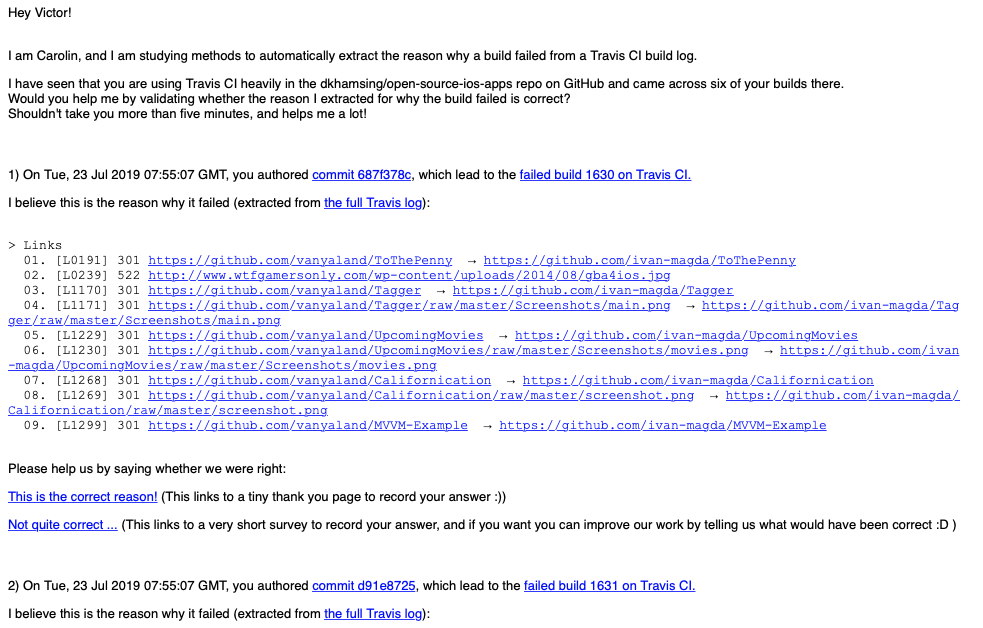
\includegraphics[width=\textwidth, clip]{img/dev-mail.png}
	\caption{An example of the mails we sent out to developers for validation of our labeled log part}
	\label{fig:dev-mail}
\end{figure}
\begin{figure}[h]
	\centering
	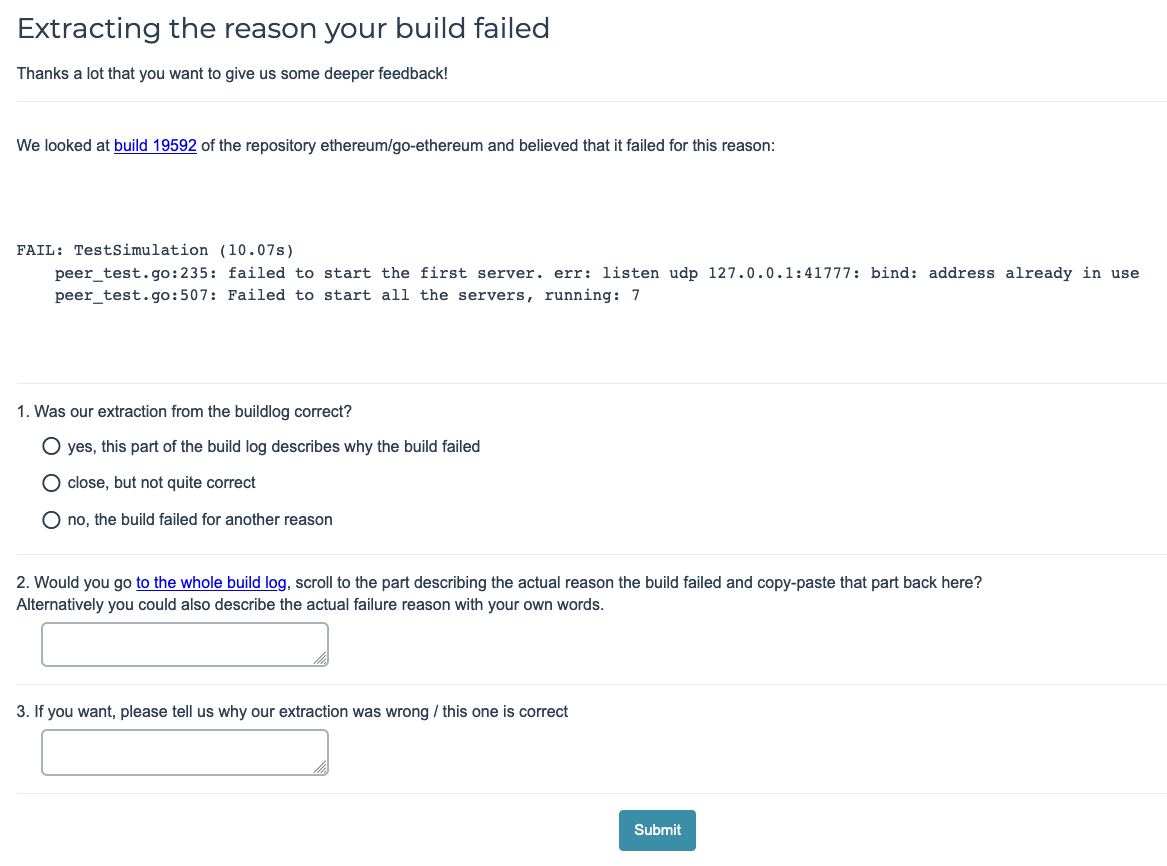
\includegraphics[width=\textwidth, clip]{img/dev-survey.png}
	\caption{Survey for the validation with developers}
	\label{fig:dev-survey}
\end{figure}


\begin{figure}[h]
	\centering
	\begin{minipage}{0.45\textwidth}
		\centering
		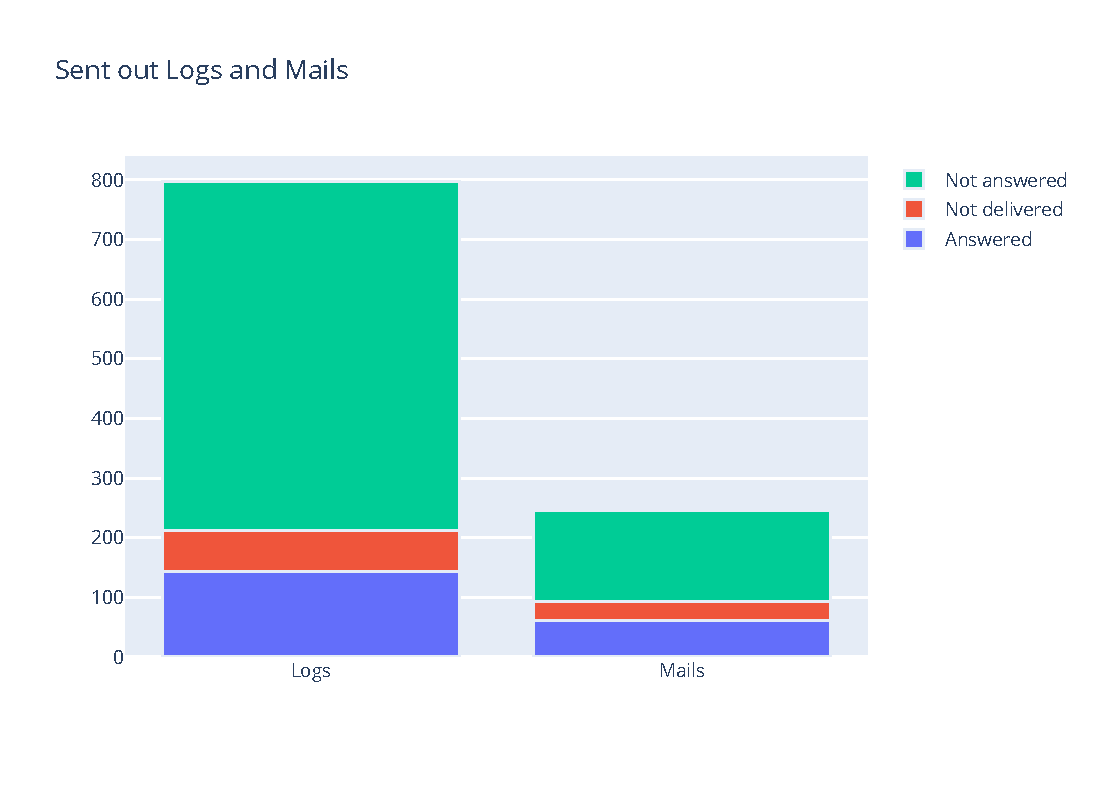
\includegraphics[width=\textwidth, clip]{img/dev-mails/answers-received.pdf}
		\caption{Proportions of Mails and Logs answered, undelivered and unanswered}
		\label{fig:mails-answers-received}
	\end{minipage}\hfill
	\begin{minipage}{0.45\textwidth}
		\centering
		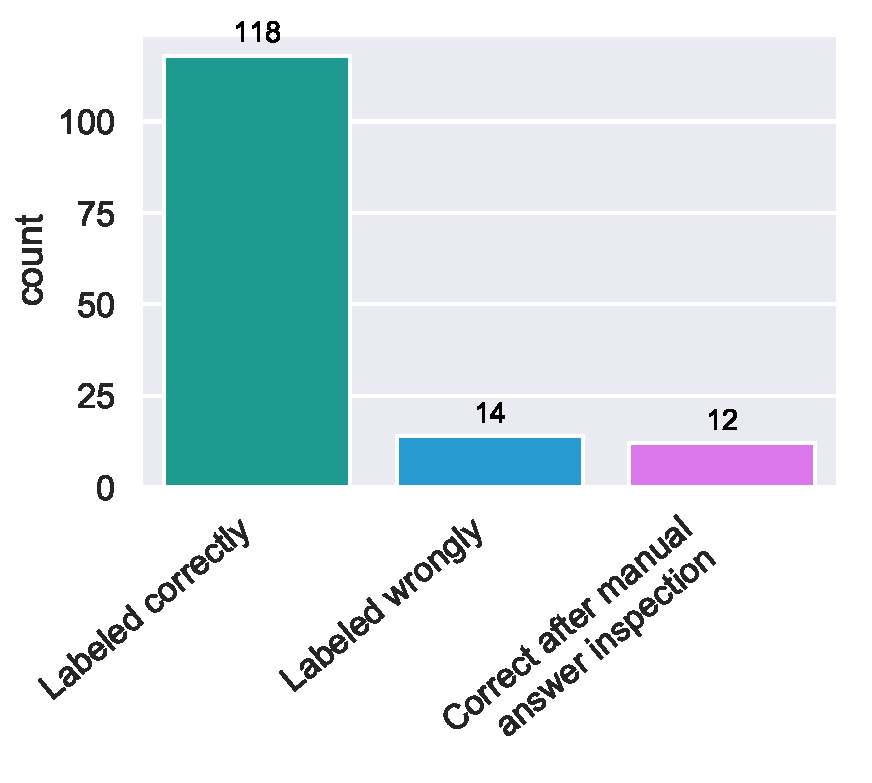
\includegraphics[width=\textwidth, clip]{img/dev-mails/extraction-correct.pdf}
		\caption{Responses to our developer survey}
		\label{fig:mails-extraction-correct}
	\end{minipage}
\end{figure}

\subsubsection{Results}
In total we sent out mails to 246 developers, asking about 3.2 build logs on average.
32 of these mails could not be delivered, e.g. because they were addressed at noreply mail addresses.
These 32 mails related to 68 of the build logs.
We received answers from 61 developers, responding about 144 build logs.
The proportions of mails and logs answered about, not delivered and unanswered is shown in Figure \ref{fig:mails-answers-received}.

Of the 144 answers, 132 said our extraction was correct.
26 answered either "close, but not quite correct" or "no, the build failed for another reason".
We manually inspected these negative answers and found that extractions were correct after all.
This yields 12 log extractions in our example set that were not correct, shown in Figure \ref{fig:mails-extraction-correct}.

\subsubsection{Discussion}
This study highly strengthens the trust in the validity of the extracted build failure reasons in the \emph{Failing Build Log Data Set}.
The study received answers about 18\% of the logs labelled in our build log, of which, after manual correction, 91\% said our labelled extractions were accurate.

Most of the initial ``incorrect'' answers we adjusted in them manual inspection, stated that the proposed extraction did not show the whole reason the build failed.
This is because we had to trim long labeled extractions to keep the emails readable.

One of our extractions only showed a warning and the developer propose to also include the line above, stating that warnings are treated as errors in the build.
In others that were identified as ``incorrect'' we labelled the error message of an error that later ignored and did not lead to the build failing.

\subsubsection{Threats to Validity}

\end{document}
